%%%%%%%%%%%%%%%%%%%%%%%%%%%%%%%%%%%%%%%%%
% Beamer Presentation
% LaTeX Template
% Version 1.0 (10/11/12)
%
% This template has been downloaded from:
% http://www.LaTeXTemplates.com
%
% License:
% CC BY-NC-SA 3.0 (http://creativecommons.org/licenses/by-nc-sa/3.0/)
%
%%%%%%%%%%%%%%%%%%%%%%%%%%%%%%%%%%%%%%%%%
%----------------------------------------------------------------------------------------
%	PACKAGES AND THEMES
%----------------------------------------------------------------------------------------

\documentclass{beamer}
\usepackage[utf8]{inputenc}
\usepackage[portuguese]{babel}
\usepackage{ragged2e}
\usepackage{multicol}
\usepackage{url}
\mode<presentation> {

% The Beamer class comes with a number of default slide themes
% which change the colors and layouts of slides. Below this is a list
% of all the themes, uncomment each in turn to see what they look like.

%\usetheme{default}
%\usetheme{AnnArbor}
%\usetheme{Antibes}
%\usetheme{Bergen}
\usetheme{Berkeley}
%\usetheme{Berlin}
%\usetheme{Boadilla}
%\usetheme{CambridgeUS}
%\usetheme{Copenhagen}
%\usetheme{Darmstadt}
%\usetheme{Dresden}
%\usetheme{Frankfurt}
%\usetheme{Goettingen}
%\usetheme{Hannover}
%\usetheme{Ilmenau}
%\usetheme{JuanLesPins}
%\usetheme{Luebeck}
%\usetheme{Madrid}
%\usetheme{Malmoe}
%\usetheme{Marburg}
%\usetheme{Montpellier}
%\usetheme{PaloAlto}
%\usetheme{Pittsburgh}
%\usetheme{Rochester}
%\usetheme{Singapore}
%\usetheme{Szeged}
%\usetheme{Warsaw}

% As well as themes, the Beamer class has a number of color themes
% for any slide theme. Uncomment each of these in turn to see how it
% changes the colors of your current slide theme.

%\usecolortheme{albatross}
% Mesma cor do trabalho original
%\usecolortheme{beaver}
%\usecolortheme{beetle}
%\usecolortheme{crane}
%\usecolortheme{dolphin}
%\usecolortheme{dove}
%\usecolortheme{fly}
%\usecolortheme{lily}
%\usecolortheme{orchid}
%\usecolortheme{rose}
%\usecolortheme{seagull}
%\usecolortheme{seahorse}
\usecolortheme{whale}
%\usecolortheme{wolverine}

%\setbeamertemplate{footline} % To remove the footer line in all slides uncomment this line
\setbeamertemplate{footline}[page number] % To replace the footer line in all slides with a simple slide count uncomment this line

%\setbeamertemplate{navigation symbols}{} % To remove the navigation symbols from the bottom of all slides uncomment this line
}
\usepackage{caption}
\usepackage{graphicx} % Allows including images
\usepackage{booktabs} % Allows the use of \toprule, \midrule and \bottomrule in tables
%----------------------------------------------------------------------------------------
%	TITLE PAGE
%----------------------------------------------------------------------------------------

\title{EP3 - Sistemas de Arquivos} % The short title appears at the bottom of every slide, the full title is only on the title page

\author{Florence Alyssa \and Shayenne Moura} % Your name
\institute[USP] % Your institution as it will appear on the bottom of every slide, may be shorthand to save space
{
Sistemas Operacionais
 \\ Bacharelado em Ciência da Computação% Your institution for the title page
\medskip
\textit{} % Your email address
}
\date{22 de novembro de 2015} % Date, can be changed to a custom date


\begin{document}

\begin{frame}
\titlepage % Print the title page as the first slide
\end{frame}

%----------------------------------------------------------------------------------------
%	PRESENTATION SLIDES
%----------------------------------------------------------------------------------------

%------------------------------------------------
\section{Introdução} 
%------------------------------------------------
\begin{frame}
\frametitle{Objetivo}
\begin{itemize}
\item Implementar um simulador de sistemas de arquivos com vários comandos que simulem ações com arquivos.
\newline

\item Linguagem: Python
\end{itemize}

\end{frame}

%------------------------------------------------
\begin{frame}
\frametitle{Suposições adotadas}
\begin{itemize}
\item Usuário comportado (não irá criar arquivos e pastas com nomes iguais)
\item 
\end{itemize}
\end{frame}

%------------------------------------------------
\section{Visão Geral} 
%------------------------------------------------
\begin{frame}
\begin{LARGE}
\begin{center}
Visão Geral
\end{center}
\end{LARGE}
\end{frame}

%------------------------------------------------
\subsection{Estrutura da Partição}
%------------------------------------------------
\begin{frame}
\frametitle{Estrutura da Partição}
\begin{figure}
\centering
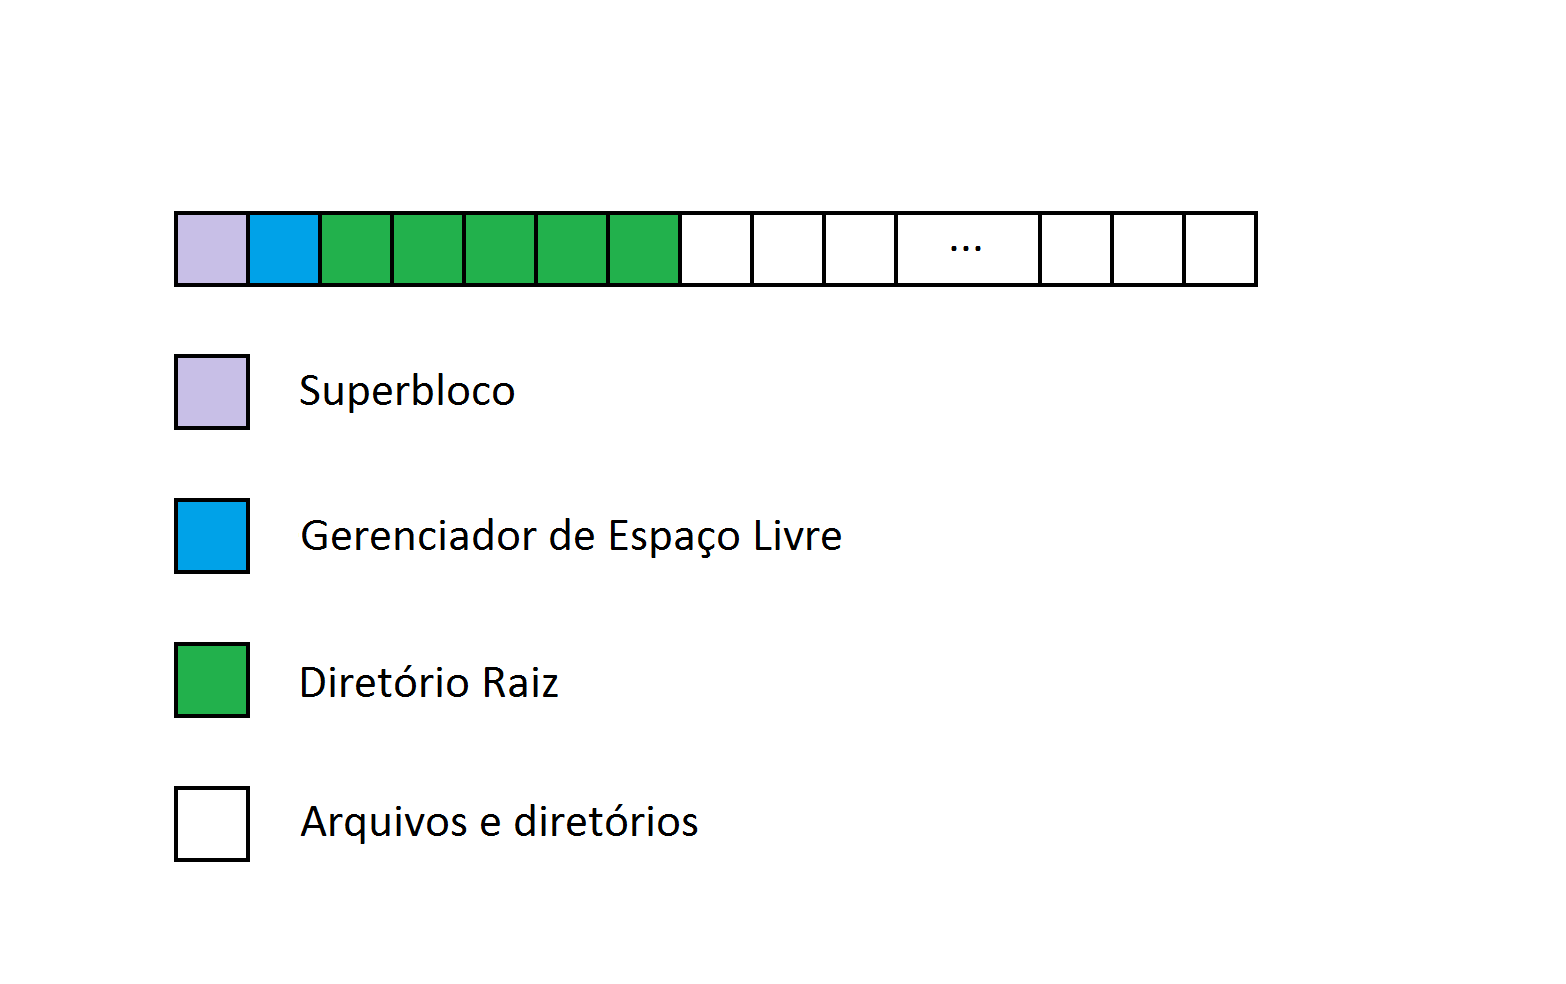
\includegraphics[scale=0.35]{particao2png.png}
\end{figure}
\justifying
\end{frame}


%------------------------------------------------
\subsection{Superbloco}
%------------------------------------------------
%------------------------------------------------
\begin{frame}
\frametitle{Superbloco}
\begin{figure}
\centering
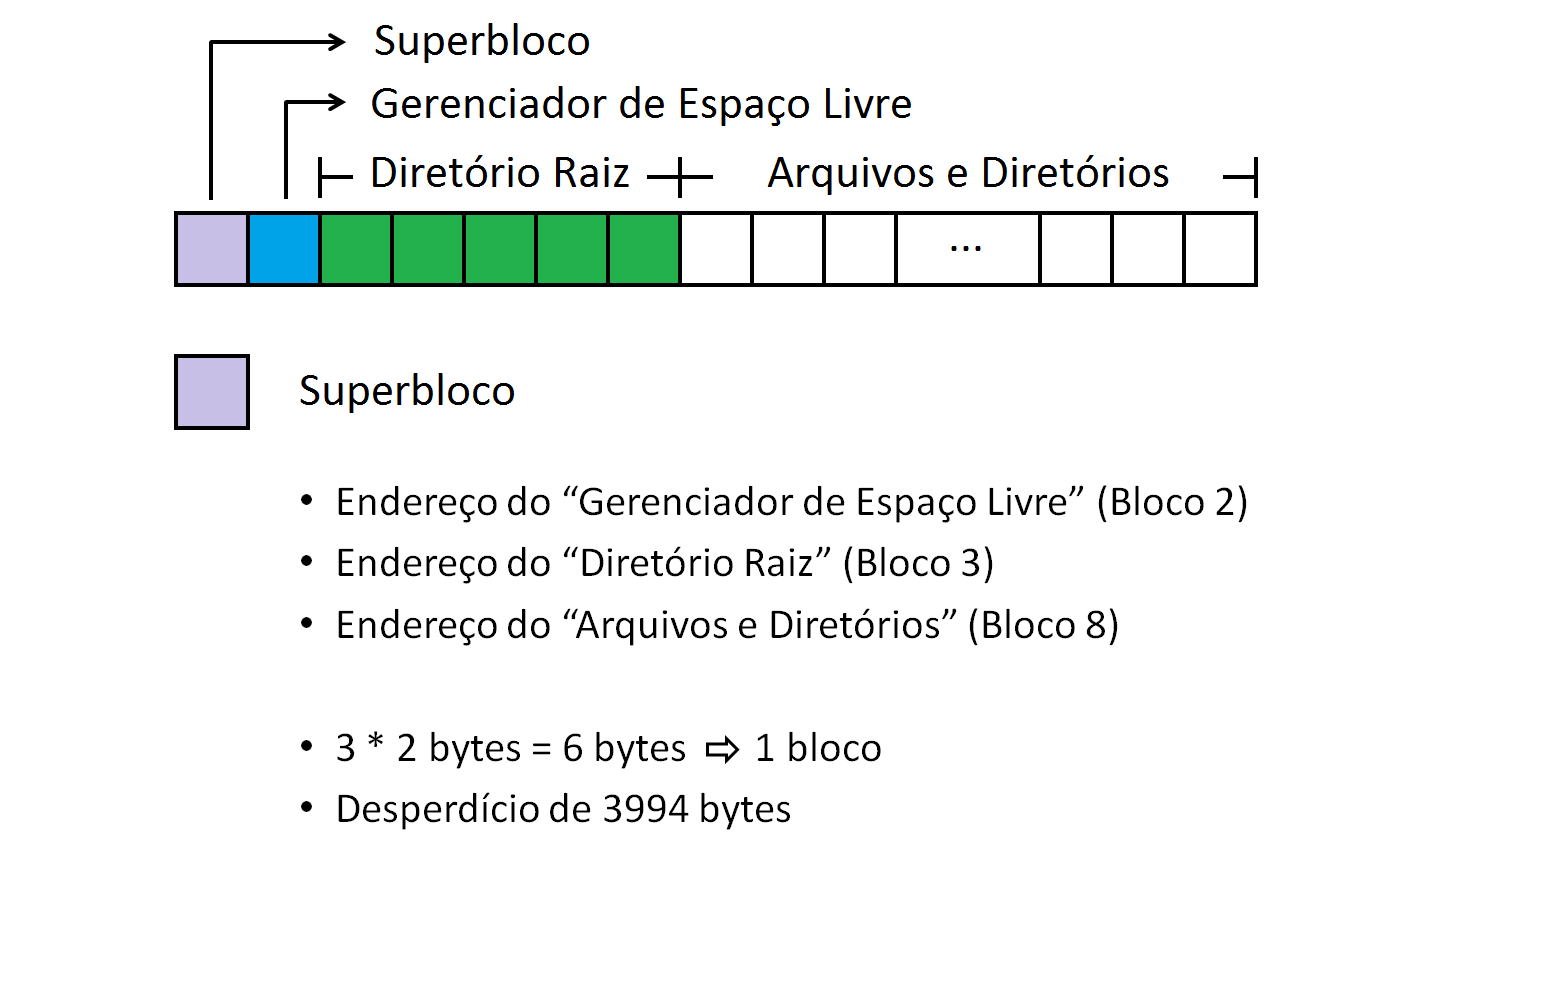
\includegraphics[scale=0.35]{superblocopng.png}
\end{figure}
\justifying
\end{frame}


%------------------------------------------------
\subsection{Gerenciador de Espaço Livre}
%------------------------------------------------
%------------------------------------------------
\begin{frame}
\frametitle{Gerenciador de Espaço Livre}
\begin{figure}
\centering
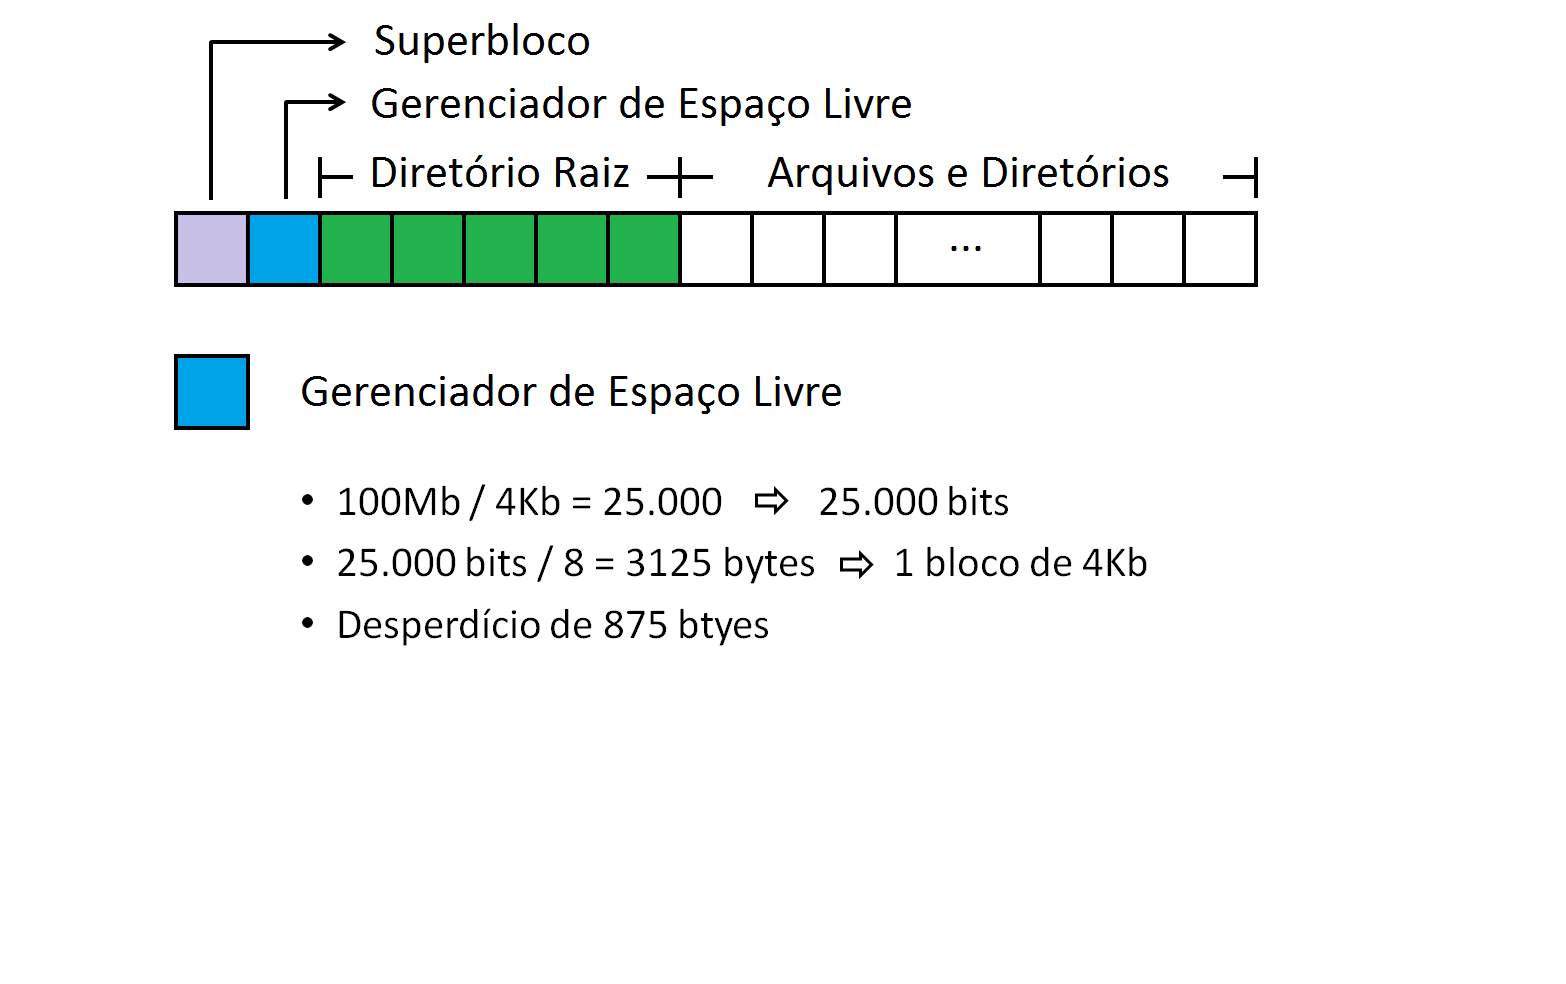
\includegraphics[scale=0.35]{gerenciadorpng.png}
\end{figure}
\justifying
\end{frame}


%------------------------------------------------
\subsection{Diretório Raiz}
%------------------------------------------------
%------------------------------------------------
\begin{frame}
\frametitle{Diretório Raiz}
\begin{figure}
\centering
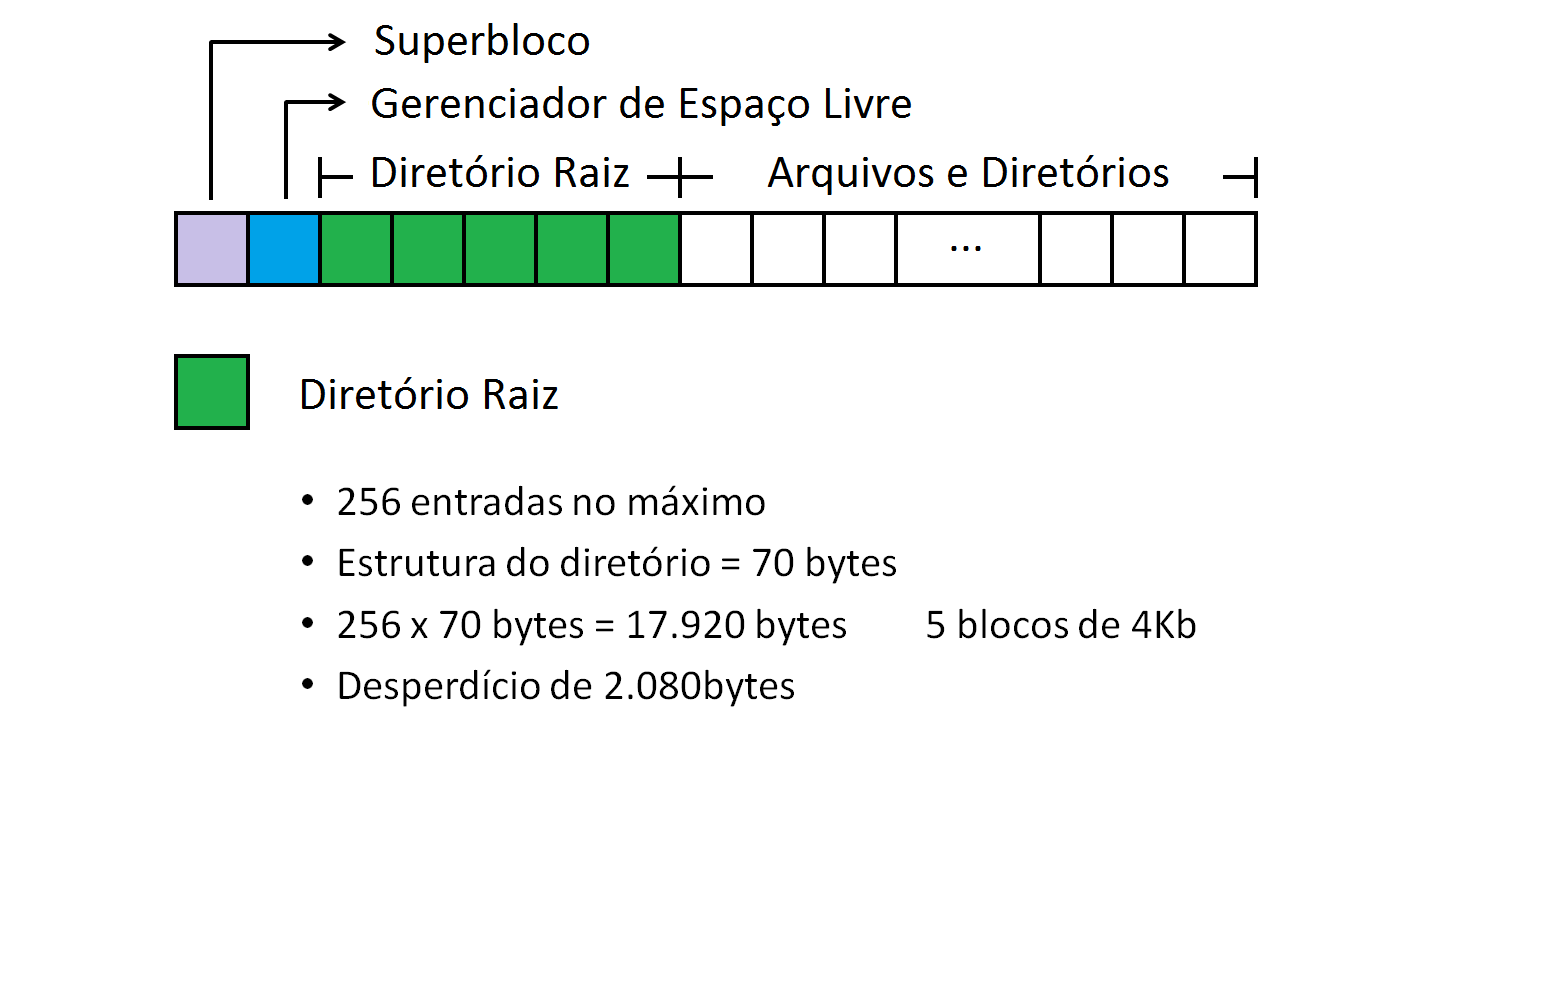
\includegraphics[scale=0.35]{raizpng.png}
\end{figure}
\justifying
\end{frame}

%------------------------------------------------
\subsection{Arquivos e Diretórios}
%------------------------------------------------
%------------------------------------------------
\begin{frame}
\frametitle{Arquivos e Diretórios}
\begin{figure}
\centering
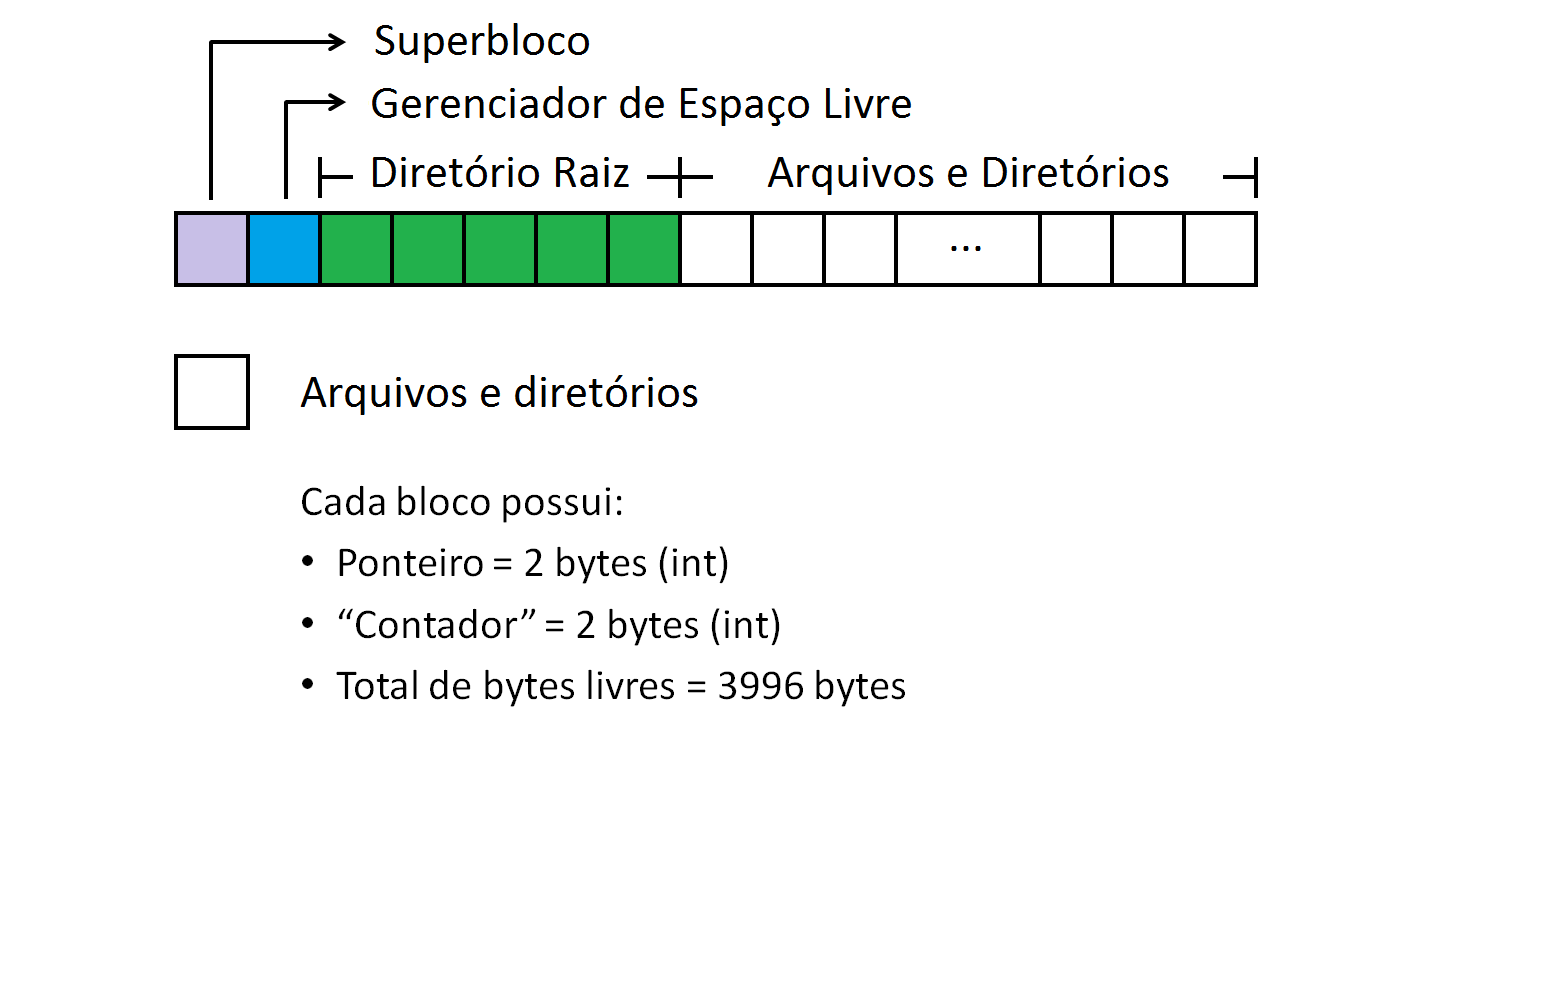
\includegraphics[scale=0.35]{arquivospng.png}
\end{figure}
\justifying
\end{frame}

%------------------------------------------------
\subsection{Atributos}
%------------------------------------------------
%------------------------------------------------
\begin{frame}
\frametitle{Atributos}
\begin{multicols}{2}

\begin{itemize}
\item Nome (12 bytes)  
\item Ponteiro (2 bytes)
\item Data: 
	\begin{itemize}
	\item Criação (16 bytes)
	\item Modificação (16 bytes)
	\item Acesso (16 bytes)
	\end{itemize}
\item Tamanho (9 bytes)
\end{itemize}

\begin{figure}
	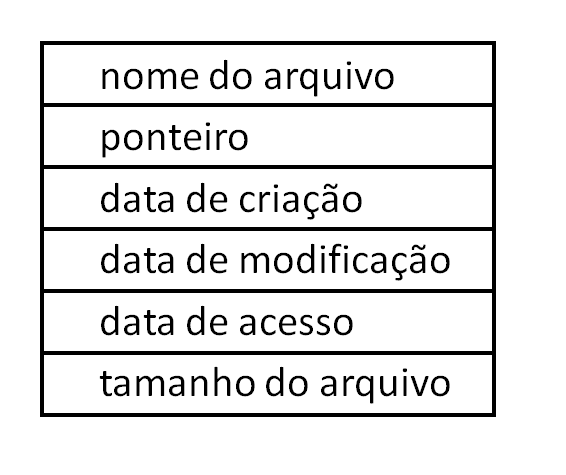
\includegraphics[scale=0.35, right]{estruturadirpng.png}
\end{figure}
\justifying
\end{multicols}

\begin{center}
[Total de 71 bytes]
\end{center}

\end{frame}


%------------------------------------------------
\section{Interação com o simulador}
%------------------------------------------------
\begin{frame}
\begin{LARGE}
\begin{center}
Interação com o simulador
\end{center}
\end{LARGE}
\end{frame}

%------------------------------------------------
%------------------------------------------------

\begin{frame}
\frametitle{Interação o simulador}


\begin{itemize}
\item mount arquivo 

\item espaço ou substitui

\end{itemize}
\end{frame}


%------------------------------------------------
%------------------------------------------------

\begin{frame}

\begin{itemize}
\frametitle{Interação o simulador}
\item executa [intervalo]

  Cria listas de espaço livre e os arquivos ep2.mem e ep2.vir preenchidos com '-1'
  
  Simula e imprime do estado da memória a cada [intervalo]s
  
\item sai

  Termina execução do simulador  

\end{itemize}
\end{frame}



%------------------------------------------------
\section{Resultados} 
%------------------------------------------------
\begin{frame}
\begin{LARGE}
\begin{center}
Resultados
\end{center}
\end{LARGE}
\end{frame}




%------------------------------------------------
\subsection{Sistema de arquivo vazio}
%------------------------------------------------
%------------------------------------------------
\begin{frame}
\frametitle{Cópia de um arquivo de 1MB no '/'} 

\justifying
\end{frame}


%------------------------------------------------
\begin{frame}
\frametitle{Cópia de um arquivo de 10MB no '/'} 

\justifying
\end{frame}


%------------------------------------------------
\begin{frame}
\frametitle{Cópia de um arquivo de 30MB no '/'} 

\justifying
\end{frame}


%------------------------------------------------
\begin{frame}
\frametitle{Remoção um arquivo de 1MB no '/'} 

\justifying
\end{frame}


%------------------------------------------------
\begin{frame}
\frametitle{Remoção um arquivo de 10MB no '/'} 

\justifying
\end{frame}


%------------------------------------------------
\begin{frame}
\frametitle{Remoção um arquivo de 30MB no '/'} 

\justifying
\end{frame}

%------------------------------------------------
\begin{frame}
\frametitle{Remoção completa com 30 níveis de hierarquia} 
Sem nenhum diretório ou arquivo regular
\justifying
\end{frame}


%------------------------------------------------
\begin{frame}
\frametitle{Remoção completa com 30 níveis de hierarquia} 
Com nenhum diretório ou arquivo regular
\justifying
\end{frame}




%------------------------------------------------
\subsection{Sistema de arquivos com 10MB ocupados}
%------------------------------------------------
%------------------------------------------------
\begin{frame}
\frametitle{Cópia de um arquivo de 1MB no '/'} 

\justifying
\end{frame}


%------------------------------------------------
\begin{frame}
\frametitle{Cópia de um arquivo de 10MB no '/'} 

\justifying
\end{frame}


%------------------------------------------------
\begin{frame}
\frametitle{Cópia de um arquivo de 30MB no '/'} 

\justifying
\end{frame}


%------------------------------------------------
\begin{frame}
\frametitle{Remoção um arquivo de 1MB no '/'} 

\justifying
\end{frame}


%------------------------------------------------
\begin{frame}
\frametitle{Remoção um arquivo de 10MB no '/'} 

\justifying
\end{frame}


%------------------------------------------------
\begin{frame}
\frametitle{Remoção um arquivo de 30MB no '/'} 

\justifying
\end{frame}

%------------------------------------------------
\begin{frame}
\frametitle{Remoção completa com 30 níveis de hierarquia} 
Sem nenhum diretório ou arquivo regular
\justifying
\end{frame}


%------------------------------------------------
\begin{frame}
\frametitle{Remoção completa com 30 níveis de hierarquia} 
Com nenhum diretório ou arquivo regular
\justifying
\end{frame}



%------------------------------------------------
\subsection{Sistema de arquivos com 50MB ocupados}
%------------------------------------------------
%------------------------------------------------
\begin{frame}
\frametitle{Cópia de um arquivo de 1MB no '/'} 

\justifying
\end{frame}


%------------------------------------------------
\begin{frame}
\frametitle{Cópia de um arquivo de 10MB no '/'} 

\justifying
\end{frame}


%------------------------------------------------
\begin{frame}
\frametitle{Cópia de um arquivo de 30MB no '/'} 

\justifying
\end{frame}


%------------------------------------------------
\begin{frame}
\frametitle{Remoção um arquivo de 1MB no '/'} 

\justifying
\end{frame}




%------------------------------------------------
%------------------------------------------------
\begin{frame}
\frametitle{Remoção um arquivo de 50MB no '/'} 

\justifying
\end{frame}


%------------------------------------------------
\begin{frame}
\frametitle{Remoção um arquivo de 30MB no '/'} 

\justifying
\end{frame}

%------------------------------------------------
\begin{frame}
\frametitle{Remoção completa com 30 níveis de hierarquia} 
Sem nenhum diretório ou arquivo regular
\justifying
\end{frame}


%------------------------------------------------
\begin{frame}
\frametitle{Remoção completa com 30 níveis de hierarquia} 
Com nenhum diretório ou arquivo regular
\justifying
\end{frame}


%------------------------------------------------
\section{Experimentos}
%------------------------------------------------
\begin{frame}
\begin{LARGE}
\begin{center}
Experimentos
\end{center}
\end{LARGE}
\end{frame}


%------------------------------------------------
\begin{frame}
\frametitle{Cópia de um arquivo de 1MB no '/'} 

\justifying
\end{frame}


%------------------------------------------------
\begin{frame}
\frametitle{Cópia de um arquivo de 10MB no '/'} 

\justifying
\end{frame}


%------------------------------------------------
\begin{frame}
\frametitle{Cópia de um arquivo de 30MB no '/'} 

\justifying
\end{frame}


%------------------------------------------------
\begin{frame}
\frametitle{Remoção um arquivo de 1MB no '/'} 

\justifying
\end{frame}

%------------------------------------------------
\begin{frame}
\frametitle{Remoção um arquivo de 10MB no '/'} 

\justifying
\end{frame}

%------------------------------------------------
\begin{frame}
\frametitle{Remoção um arquivo de 30MB no '/'} 

\justifying
\end{frame}

%------------------------------------------------
\begin{frame}
\frametitle{Remoção completa de um diretório pai com 30 níveis de hierarquia} 
VAZIA
\justifying
\end{frame}


%------------------------------------------------
\begin{frame}
\frametitle{Remoção completa de um diretório pai com 30 níveis de hierarquia} 
CENTENAS DE ARQUIVOS
\justifying
\end{frame}




%------------------------------------------------
%------------------------------------------------
\begin{frame}
\frametitle{Remoção um arquivo de 50MB no '/'} 

\justifying
\end{frame}


%------------------------------------------------
\begin{frame}
\frametitle{Remoção um arquivo de 30MB no '/'} 

\justifying
\end{frame}

%------------------------------------------------
\begin{frame}
\frametitle{Remoção completa com 30 níveis de hierarquia} 
Sem nenhum diretório ou arquivo regular
\justifying
\end{frame}


%------------------------------------------------
\begin{frame}
\frametitle{Remoção completa com 30 níveis de hierarquia} 
Com nenhum diretório ou arquivo regular
\justifying
\end{frame}


\end{document}
